\chapter{Related Work}
\label{chap:RelatedWork}
\index{Related Work}

%%%%%%%%%%%%%%%%%%%%%%%%%%%%%%%%%%%%%%%%%%%%%%%%%%%%%%%%%%%%%%%%%%%%%%%%%%%%%%%%

As discussed in the previous chapter, we split our work into two parts:
(1) person re-identification (2) device abstraction.
In this chapter, we are going to introduce the background for each part. For the
person re-identification part, we will review the literature related to object
detection and person re-identification, which the former is a prerequisite of
the latter. For the device abstraction part, we are going to examine currently
available software which may become useful for our objectives and be adopted as
dependencies in our solution.


\section{Object Detection}
\label{sec:related_work_obj_det}

Object detection is one of the fundamental tasks in computer vision research.
It is a natural extension of the classification problem that requires the 
detection of
the presence of objects and to accurately locate them within the given image.
This subject has been explored by many researchers for a long time and a lot of
detailed surveys have been published on this topic
\cite{survey2-on-dl-od-2018, survey1-on-dl-od-2018}.
We can observe from \autoref{fig:od-timeline}, since 2012 the deep
learning-based approaches have dominated the object detection domain.
In this section, we are going to review the two classes of literature in object
detection based on deep learning methods (detailed explanation will be given as
subsection for each of the items listed below).

\pagebreak

\begin{itemize}
    \item Two stages approaches
    \begin{itemize}
        \item \acrshort{rcnn}
        \item \acrshort{sppnet}
        \item Fast R-CNN
        \item Faster R-CNN
        \item Mask R-CNN
    \end{itemize}

    \item One stage approaches
    \begin{itemize}
        \item \acrshort{yolo} v1, v2 and v3
        \item \acrshort{ssd}
    \end{itemize}
\end{itemize}

\begin{figure}
    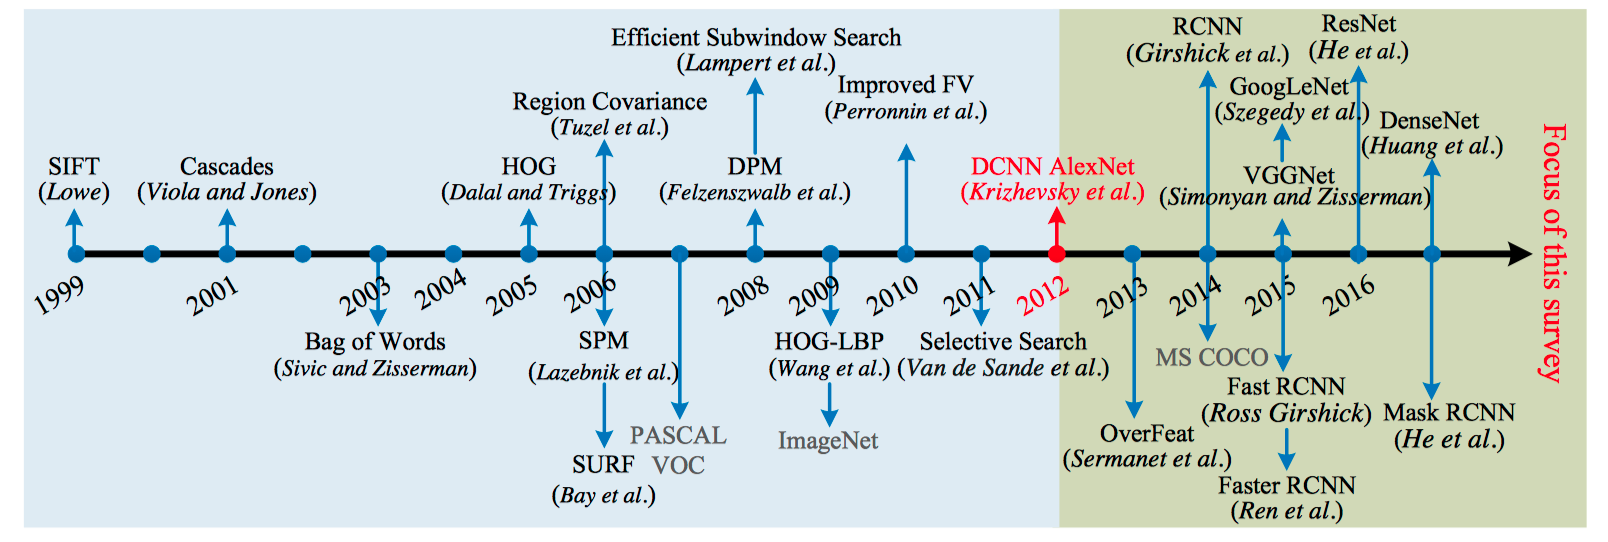
\includegraphics[width=\linewidth]{figures/timeline_od.png}
    \caption[Timeline of various methods proposed for object detection]
    {Timeline of various methods proposed for object detection
    ~\protect\cite{survey1-on-dl-od-2018}. The methods in blue area are the
    hand-crafted detector and those in green area are the deep
    learning-based approaches.}
    \label{fig:od-timeline}
\end{figure}

The world ``stage'' here means an independent process or a separate branch
within the deep neural network structure.
As their names imply, one-stage approaches finish the whole object detection
process in one shot
%indicating it will be faster than its two stages sibling
%due to the fact that less computation being performed.
while the two-stages approach has an independent process to propose the areas
that may contain an object then perform detection on those areas. The
presence of the area proposition stage takes more time but since it is 
elaborated and can cover more potential areas than the one-stage approach, it 
can achieve better results in terms of accuracy.
To determine which kind of detector to use depends on the realistic
requirement of the application. In this thesis, since we have real-time response
as a non-functional requirement, one stage detector will definitely be a better 
choice. 
%and we mainly focus on the YOLO v3 detector, the implementation detail will be 
%explained in the next chapter.

\subsection{Two Stages Detector}
\label{sec:related-worked-two-stages-detector}

Most of the two stages detectors follow the same methodology. Firstly,
propose candidate regions that may contain object(s) then using a
convolutional neural network (\acrshort{cnn}) to extract feature descriptors of 
each region.
Finally, feed the descriptor into a classifier to figure out what kind of 
object they are if it exists, and classify them according to a set of 
pre-defined categories.

\subsubsection{R-CNN}

R-CNN was the seminal work of employing CNN on object detection task, the name 
R-CNN stands for region with CNN features. At the
time it was proposed, it boosted the accuracy from 35.1\% to 53.7\% on PASCAL
VOC dataset \cite{r-cnn-paper-2013}.
It designed a cascade pipeline containing four modules shown as
\autoref{fig:r-cnn}.
There are two important points this work brought to the table:
(1) it proposed a selective search 
\footnote{Selective Search is a region 
proposal algorithm used in object detection. It is designed to be fast with a 
very high recall. It is based on computing hierarchical grouping of similar 
regions based on color, texture, size and shape compatibility.} 
method to find the possible candidates
replacing the old fashion sliding window method,
which improves the computation time significantly.
(2) it adopted CNN as a feature extractor which yields more robust
features rather than the hand-crafted one.

\begin{figure}
    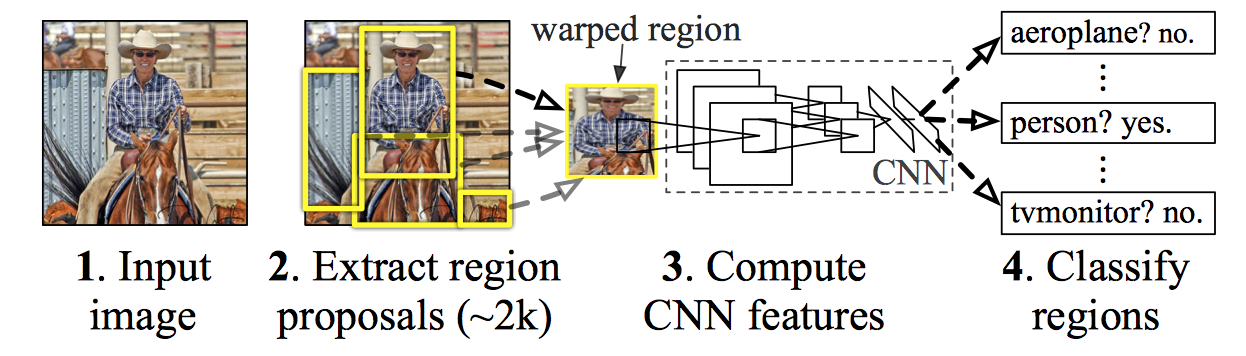
\includegraphics[width=\linewidth]{figures/r_cnn.png}
    \caption{R-CNN system overview ~\protect\cite{r-cnn-paper-2013}.}
    \label{fig:r-cnn}
\end{figure}

\subsubsection{SPP-net}

Even though R-CNN brought a large margin of improvement into object detection
research, it still has the potential to be better, as observed by Kaiming He and
his team. They proposed spatial pyramid pooling network (SPP-net)
\cite{spp-net-paper-2014} one year after the publication of R-CNN. It improved
both runtime efficiency and accuracy compared to R-CNN.
They identified two main issues in the R-CNN solution:

\begin{itemize}
    \item The generated candidate regions are easy to have overlap among each 
    other which can lead to repeated computation of the same feature maps.

    \item When ensuring the input image to a fixed size by cropping or
    warping, it may leads to information
    missing which can affect the training significantly.
\end{itemize}

SPP-net solved the first problem by reversing the order of selective search and
convolution operation.
It also employed a special layer named ``spatial pyramid pooling" at the
end of the convolutional layer to eliminate the second problem, that is how its 
name comes from.
By using SPP-net, the final feature maps will only be
computed once and the features are pooled in arbitrary regions to generate 
fixed-length descriptor for training, as shown in \autoref{fig:spp-net}.


\begin{figure}
    \begin{center}
    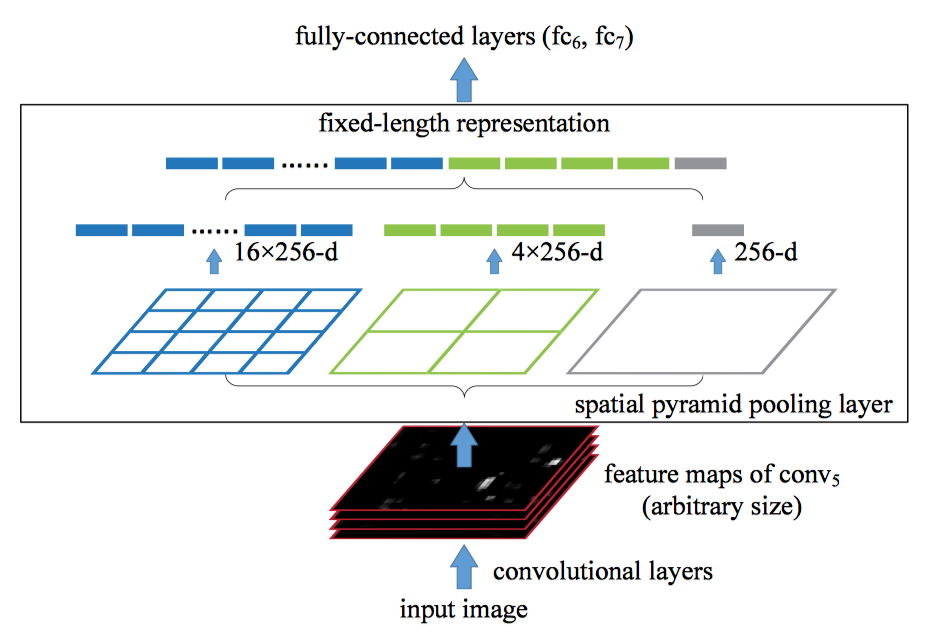
\includegraphics[scale=0.7]{figures/spp_net.png}
    \end{center}
    \caption{Illustration of how spatial pyramid layer works
    ~\protect\cite{spp-net-paper-2014}.}
    \label{fig:spp-net}
\end{figure}


\subsubsection{Fast R-CNN}

Fast R-CNN \cite{fast-r-cnn-paper-2015}, as its name suggests, is
a performance-enhanced version of R-CNN.
This update mainly focuses on speeding up both
training and testing procedures. It targeted its improvements
at not only R-CNN but also SPP-net for their common drawbacks:

\begin{itemize}
    \item The training pipeline is a multi-stage process.
    \item Features are written to disk during training.
    \item The inference phase is too slow.
\end{itemize}

The solution for these issues is quite straightforward. Firstly, the author
changed the cascade pipeline to become a parallel one, shown as
\autoref{fig:fast-r-cnn}. 
Secondly, it modified the loss to be a multi-task loss which reduces the
training complexity and makes all the layers updatable (the proposed fine-tuning
algorithm cannot update the convolutional layer that precedes the spp layer).
Thirdly, the features cached on the disk were no longer needed.

\begin{figure}
    \begin{center}
    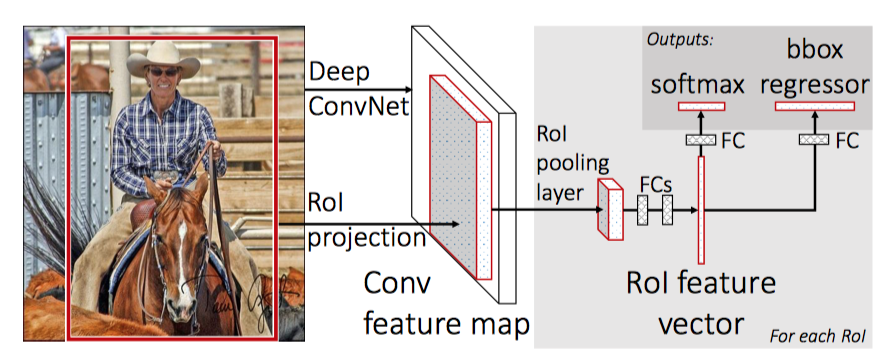
\includegraphics[scale=0.7]{figures/fast_r_cnn.png}
    \end{center}
    \caption{Parallel workflow of Fast R-CNN
    ~\protect\cite{fast-r-cnn-paper-2015}.}
    \label{fig:fast-r-cnn}
\end{figure}


\subsubsection{Faster R-CNN}

Faster R-CNN \cite{faster-r-cnn-paper-2015} was a milestone of the usage of 
deep convolutional neural network in the research of object detection. It was 
created by the combination of the teams which proposed R-CNN and SPP-net.
Before it came up, the candidate regions were calculated via a method called 
selective search. 
But in this case, they introduced a region proposal network (RPN) which was 
embedded as a branch into the model that can learn how to
produce reliable candidate regions during the training time, the overall
structure of Faster R-CNN as shown in \autoref{fig:faster-r-cnn}.
By using such a solution, the model can achieve object bounding box prediction 
and object classification simultaneously (through one 
forward pass). There are several advantages of Faster R-CNN compared to 
previous works:

\begin{itemize}
    \item Deep learning features are more reliable than the selective search one.
    \item The whole network can be trained end-to-end \footnote{The learning 
    that optimizes the network weights by considering the inputs and outputs 
    directly is called end-to-end learning. }.
    \item The whole pipeline can be done on GPU (selective search need to be
    done on CPU before) which can speed up the training time.
\end{itemize}

\begin{figure}
    \begin{center}
        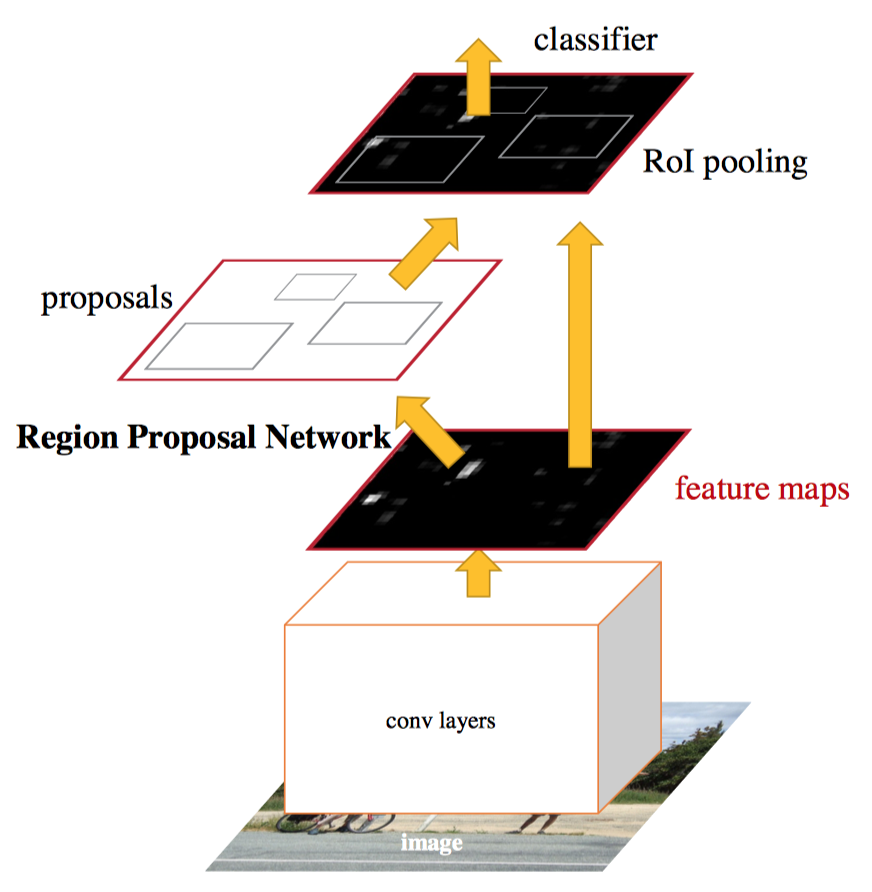
\includegraphics[scale=0.5]{figures/faster_r_cnn.png}
    \end{center}
    \caption{Structure of Faster R-CNN ~\protect\cite{faster-r-cnn-paper-2015} 
    network.}
    \label{fig:faster-r-cnn}
\end{figure}

There is one more thing that needs to be pointed out, this work introduced the
concept of ``anchor'' which has been widely
used in the latter object detection research including the one stage
detector we are going to review in the next subsection.
At each sliding-window position, the network would simultaneously predict $k$
region proposals relative to
$k$ reference bounding boxes. These reference boxes are called anchor, an 
example of which is shown in \autoref{fig:anchor}.

\begin{figure}
    \begin{center}
    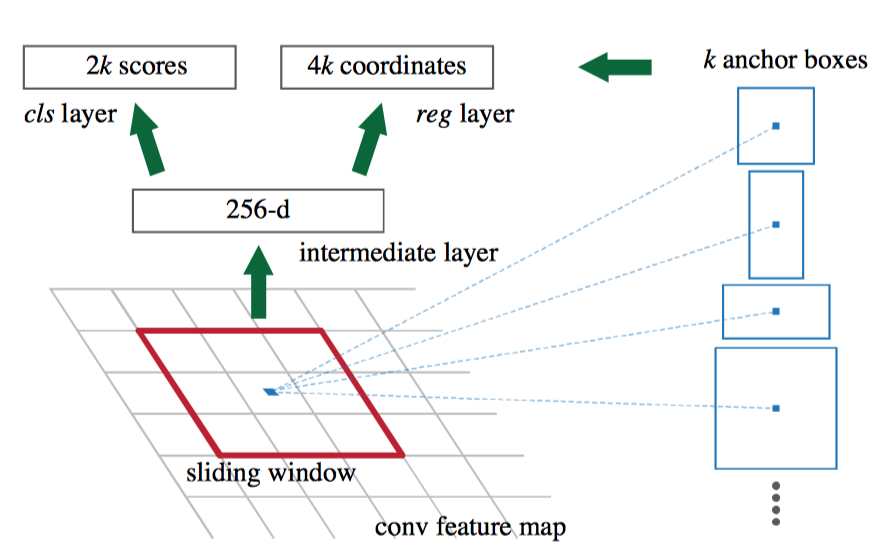
\includegraphics[scale=0.6]{figures/anchor.png}
    \end{center}
    \caption{Illustration of the anchor mechanism
    ~\protect\cite{faster-r-cnn-paper-2015}.}
    \label{fig:anchor}
\end{figure}


\subsubsection{Mask R-CNN}

The most recent work of the R-CNN-based research, called Mask
R-CNN \cite{mask-r-cnn-paper-2017}, was proposed
by Kaiming He again. It was an object detection network also which could be
used in the object segmentation domain. The idea
was that (1) it added another mask branch into the network to create a mask for
each detected object instance and (2) it used a
more advanced backbone network for feature extraction (e.g. ResNet and FPN).
Its architecture is shown in \autoref{fig:mask-r-cnn}.
Again, the loss used to guide the training is the multi-task loss from Faster
R-CNN with the mask loss added, expressed as:
$L = L_{cls} + L_{bbox} + L_{mask}$. Another creative idea, ROI alignment, is
notable to mention which can improve accuracy for bounding boxes regression.

\begin{figure}
    \begin{center}
    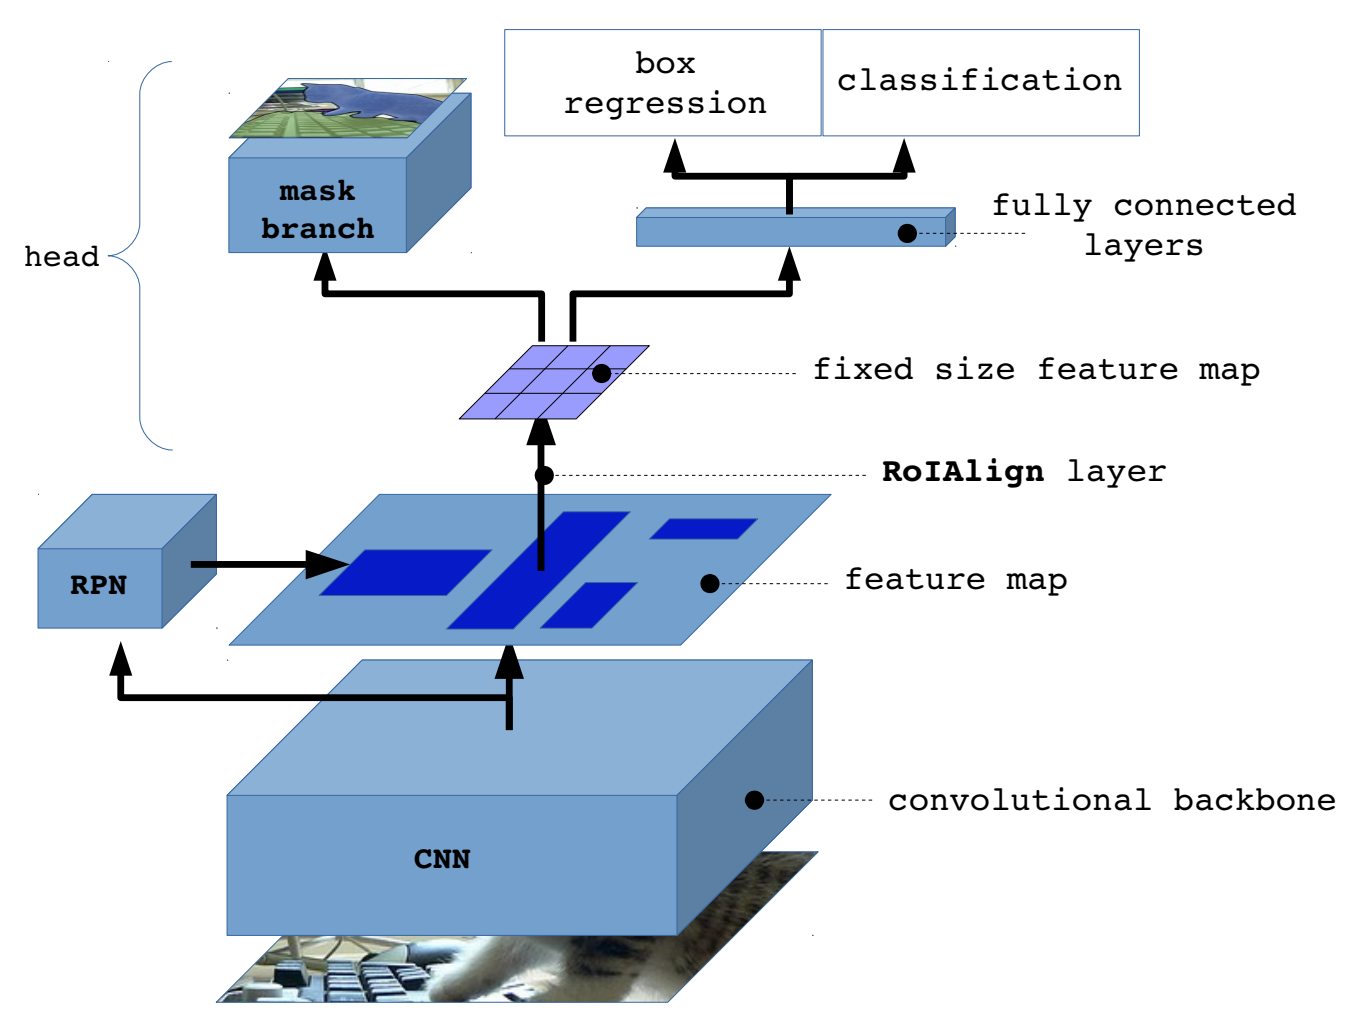
\includegraphics[scale=0.5]{figures/mask_r_cnn.png}
    \end{center}
    \caption{Architecture of Mask R-CNN ~\protect\cite{mask-r-cnn-slide}.}
    \label{fig:mask-r-cnn}
\end{figure}


\subsection{One Stage Detector}
\label{sec:related-worked-one-stage-detector}

One stage detector refers to those who directly predict classification score and bounding
box offsets from the input with a single feed-forward CNN network. There is no
separate region proposition process that exists at all. All the computation is done
within just a single network which can be optimized end-to-end directly on
detection performance.

\subsubsection{YOLO}
\label{sec:related-worked-yolo}

YOLO stands for ``you only look once'', which indicates it is an one-stage
object detector. Until now, there is a total of 
three versions of the YOLO algorithm. They are YOLO v1, YOLO v2, YOLO v3 which 
were published in 2015, 2016, 2018 respectively. 
Compared with the R-CNN series, YOLO doesn't have the stage of 
candidate region calculation. It uses a single network to
directly compute the object classification score and regress the bounding
boxes if the object exists.

\textbf{YOLO v1} \cite{yolov1-paper-2015}, this work is the fundamental
building block. The latter YOLO algorithms
just borrowed or added advanced techniques or tricks to improve the
performance. The workflow of the algorithm can
be summarized as the following steps and visualized as
\autoref{fig:yolo-v1-workflow}:

\begin{itemize}
    \item Take the input image (with size $448 \times 448$), cut it into $S
    \times S$ grids, each of them is responsible for detecting those objects
    whose center located within this grid.

    \item Each grid will predict $B$ (an integer) bounding boxes and the
    confidence score of each box. For each predictive bounding box, the result
    should be a five-dimensional vector $(x, y, w, h, c)$ representing the 
    center location of the box $(x, y)$, the width and height of the box $(w, 
    h)$, and the confidence score $c$.

    \item For each grid (no matter how many bounding boxes are required), it should
    also output a probability for all required classes (if the dataset contains
    10 classes of object, it should output a probability for each class which
    means 10 probabilities in total).

    \item Sort all the results according to the score and use a threshold to 
    filter out the detected bounding boxes whose probability is lower than the 
    threshold.
\end{itemize}

\begin{figure}
    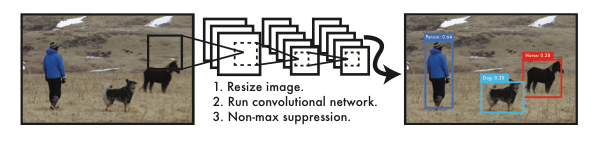
\includegraphics[width=\linewidth]{figures/yolo_v1_workflow.png}
    \caption{Workflow of YOLO v1 ~\protect\cite{yolov1-paper-2015}.}
    \label{fig:yolo-v1-workflow}
\end{figure}

An example process for an input image can be shown as
\autoref{fig:yolo-v1-example}. From that figure we can find that the
classification score computation and bounding box prediction happened in
parallel. At
the end, another common technique, non-maximum
suppression \cite{non-maximum-suppression-paper} was applied to eliminate the
highly overlapped boxes but point to the same object.
From the implementation point of view, the YOLO series was written in pure C. 
The author provided his own deep learning framework
named Darknet \cite{darknet13} which includes
backbone network, optimizer, parameters update
methods, etc. The backbone network's architecture is shown as
\autoref{fig:yolo-network}, which is a 24 convolutional layers network
with 2 dense layers appended. The whole model was pre-trained on ImageNet
using image with resolution $224 \times 224$ then doubled the size for
detection.


\begin{figure}
    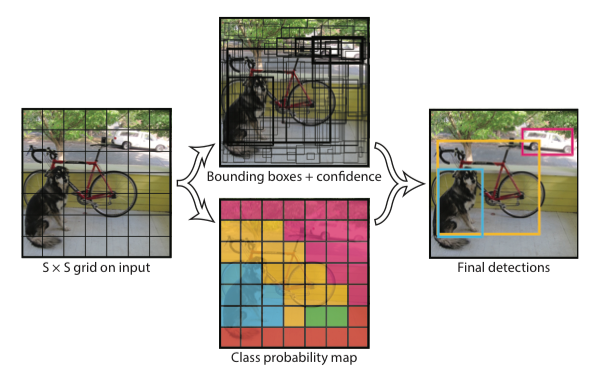
\includegraphics[width=\linewidth]{figures/yolo_v1_grid_example.png}
    \caption{Process example YOLO v1 ~\protect\cite{yolov1-paper-2015}.}
    \label{fig:yolo-v1-example}
\end{figure}

\begin{figure}
    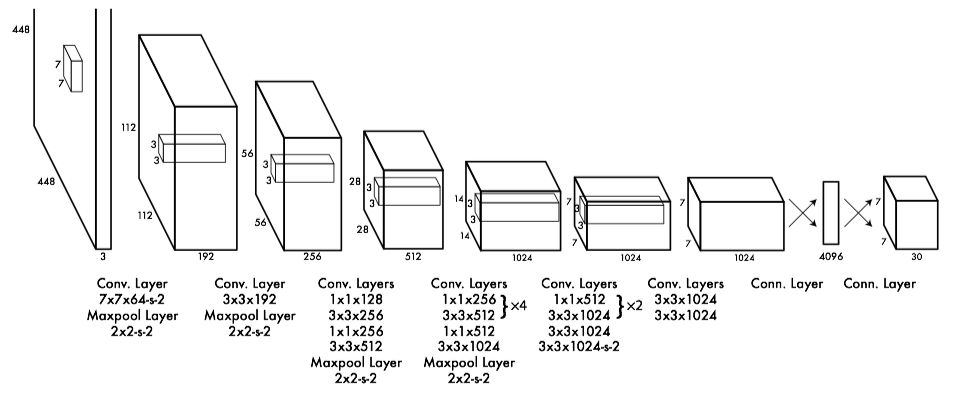
\includegraphics[width=\linewidth]{figures/yolo_v1_network_architecture.png}
    \caption{YOLO v1 network architecture ~\protect\cite{yolov1-paper-2015}.}
    \label{fig:yolo-network}
\end{figure}

\textbf{YOLO v2} \cite{yolov2-paper-2016} is an update of the
previous version to improve the performance while
keeping its speed advantage (67 FPS vs. 5 FPS for Faster R-CNN).
A comparison result with other detector can be found in 
\autoref{fig:yolo-v2-s-acc}. The development efforts have been concentrated on:

\begin{itemize}
    \item Added batch normalization layer to gain 2\% improvement in the 
    context of mAP .

    \item Pre-train on ImageNet using images with size $448 \times
    448$ (double compared to YOLO v1) which increases 4\% mAP.

    \item Introduced ``anchor mechanism'' from Faster R-CNN which
    bring 7\% recall improvement.

    \item During training, every 10 epochs change the scale of images to obtain
    more powerful generalization ability.

    \item $13 \times 13$ resolution feature map is enough for ordinary objects
    but in order to overcome the disadvantage from v1 that perform poorly on
    small objects, a passthrough layer has been added that bring the feature
    from an earlier layer at $26 \times 26$ resolution.

    \item Proposed a new backbone network called Darknet-19 which contains 19
    convolutional layers and 5 maxpooling layers.
\end{itemize}

\begin{figure}
    \begin{center}
    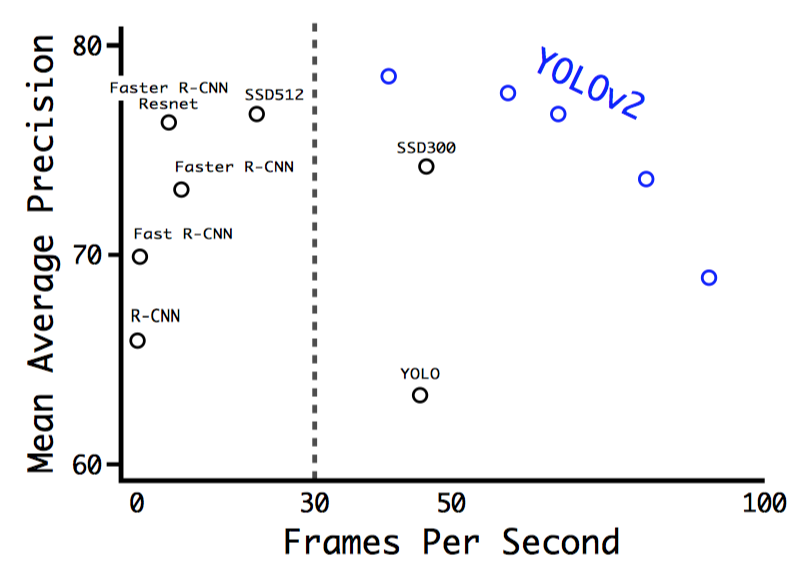
\includegraphics[scale=0.7]{figures/yolov2_speed_and_acc.png}
    \end{center}
    \caption{YOLO v2 accuracy and speed on VOC 2007 dataset
    ~\protect\cite{yolov2-paper-2016}.}
    \label{fig:yolo-v2-s-acc}
\end{figure}

\textbf{YOLO v3} \cite{yolov3-paper-2018}, the author tried a number of tricks 
and found some of them can increased the speed and accuracy.
A comparison of the inference time between YOLO v3 and most of considerable 
methods can be shown as \autoref{fig:yolo-v3-comp}.
According to their paper, some significant changes have been applied in this
version:

\begin{itemize}
    \item It used a new backbone classification network design based on the
    works of Residual Network \cite{resnet-paper1-2015}
    \cite{resnet-paper2-2016} named Darknet-53 which can improve the top1
    accuracy about 3.1\% while maintaining the speed of 78 FPS.

    \item It discarded the softmax function for classification instead using a 
    simple logistic classifier. 
    During the training, binary cross-entropy loss was
    employed which can solve the problem of overlapping labels (i.e. man and
    person) in a complex dataset.

    \item It adopted a similar concept of feature pyramid networks (FPN) to
    enhance the scale-invariant ability of the model.
\end{itemize}

\begin{figure}
    \begin{center}
        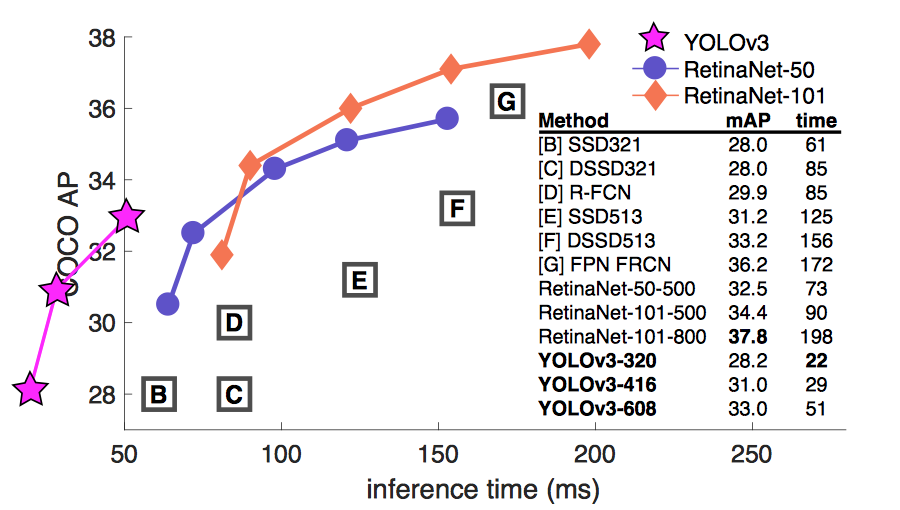
\includegraphics[scale=0.7]{figures/yolov3_comp.png}
    \end{center}
    \caption{Inference time of YOLO v3 compared with other methods
        ~\protect\cite{focal-loss-for-dense-od}.}
    \label{fig:yolo-v3-comp}
\end{figure}

\subsubsection{SSD}

Five months after YOLO v1 was published, another famous one-stage approach,
named single shot detector (SSD) was created \cite{ssd-paper-2015}. 
It achieved much higher performance on mAP metric than YOLO v1, precisely, 
72.1\% mAP on VOC2007 dataset at 58 FPS with $300 \times 300$ input size while 
YOLO v1 only have 63.4 \% at 45 PFS with
$448 \times 448$ input size. The architecture difference between YOLO v1 and 
SSD can be shown by \autoref{fig:ssd_yolo_net}.
This performance increase can be explained by the following improvements:

\begin{itemize}
    \item Use of the ``anchor mechanism'' to find a set of pre-defined bounding boxes.

    \item For each anchor, predict the class label and the offset of the
    anchor which perform better than regress the absolute location of the 
    bounding box.

	\item For each input, combine feature maps with different scales in order to
    achieve scale invariant.
\end{itemize}

\begin{figure}
    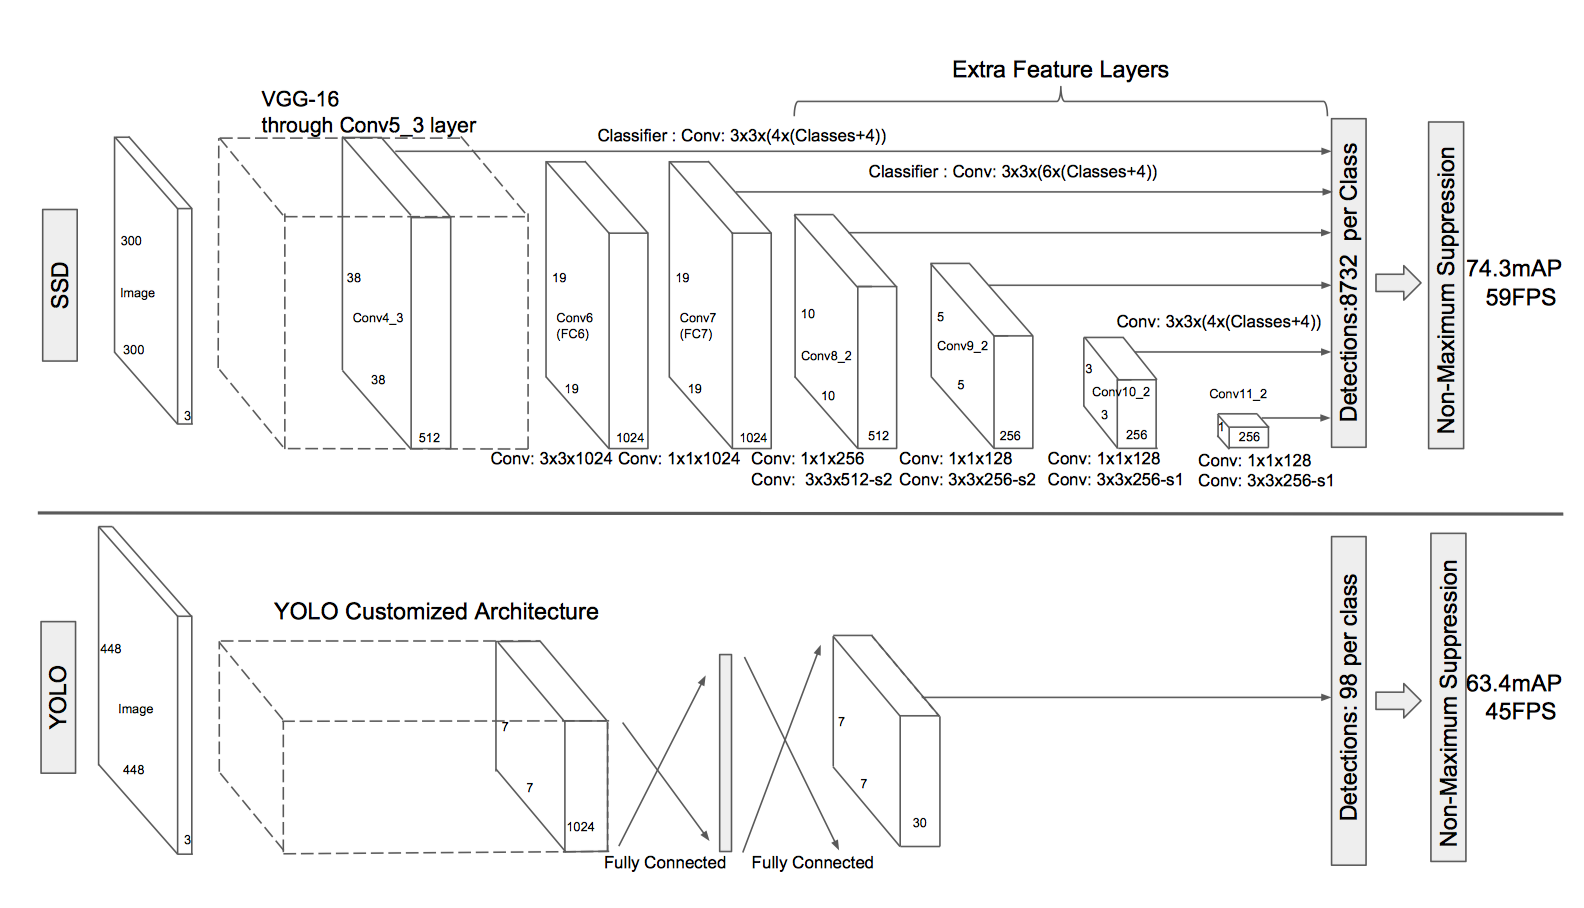
\includegraphics[width=\linewidth]{figures/ssd_yolo_net_arch.png}
    \caption{Network architecture comparison between SSD and YOLO v1
    ~\protect\cite{ssd-paper-2015}.}
    \label{fig:ssd_yolo_net}
\end{figure}

\section{Person Re-Identification}
\label{sec:related_work_re_id}

%According to \cite{survey-reid-past-present-feature-2016}, the first definition
%of person re-identification was given by Alvin Plantinga in 1961, when he 
%discussed the relation between mental state and behavior. It was saying that:
%
%\begin{quotation}
%``To re-identify a particular, then, is to identify it as (numerically) the
%same particular as one encountered on a previous occasion.''
%\end{quotation}

Re-identification means we need to determine whether we encounter the same 
target on a previous occasion or not.

According to \cite{survey-on-dl-for-reid-2019}, let $\delta=\{\delta_1, ...,
\delta_M \}$ represents $M$ descriptors within a gallery set, given a probe
descriptor $U$, the identity of this probe person can be formulated as:

\begin{equation}
\label{general-reid-formula}
I = \arg_{\delta_i} \min (dis(\delta_i, U)),  \: \delta_i \in \delta
\end{equation}

\noindent 
where $I$ represent the identity of $U$ and $dis$ means a proper distance
function which will return the distance between $U$ and all $\delta_i \in 
\delta$. From \autoref{general-reid-formula}, we should notice that there are 
two key points of the person ReID task:
(1) Feature description and (2) Distance function.
How to obtain suitable feature descriptors is always an interesting research
problem in the computer vision area. The traditional way to do it through
a hand-crafted descriptor which is designed by the domain experts, for
example, BRIEF, SIFT, SURF, and ORB descriptors. All these are hand-crafted
descriptors and work well in their own domain. But for different tasks, 
different
descriptors have to be created. Obviously, it requires a lot of work and is not
very convenient.

Since 2012, AlexNet \cite{imagenet-classifi-cnn} got a huge success in the
ImageNet classification competition with the use of deep learning. Using deep
neural network as feature extractor has become popular and its performance defeats
most of the descriptors created manually. In the person ReID community, more 
and more researchers move their attention to the deep learning-based features 
(statistic shown in \autoref{fig:papers-trend}) and a lot of creative methods 
have been developed based on (deep) neural networks.

\begin{figure}
    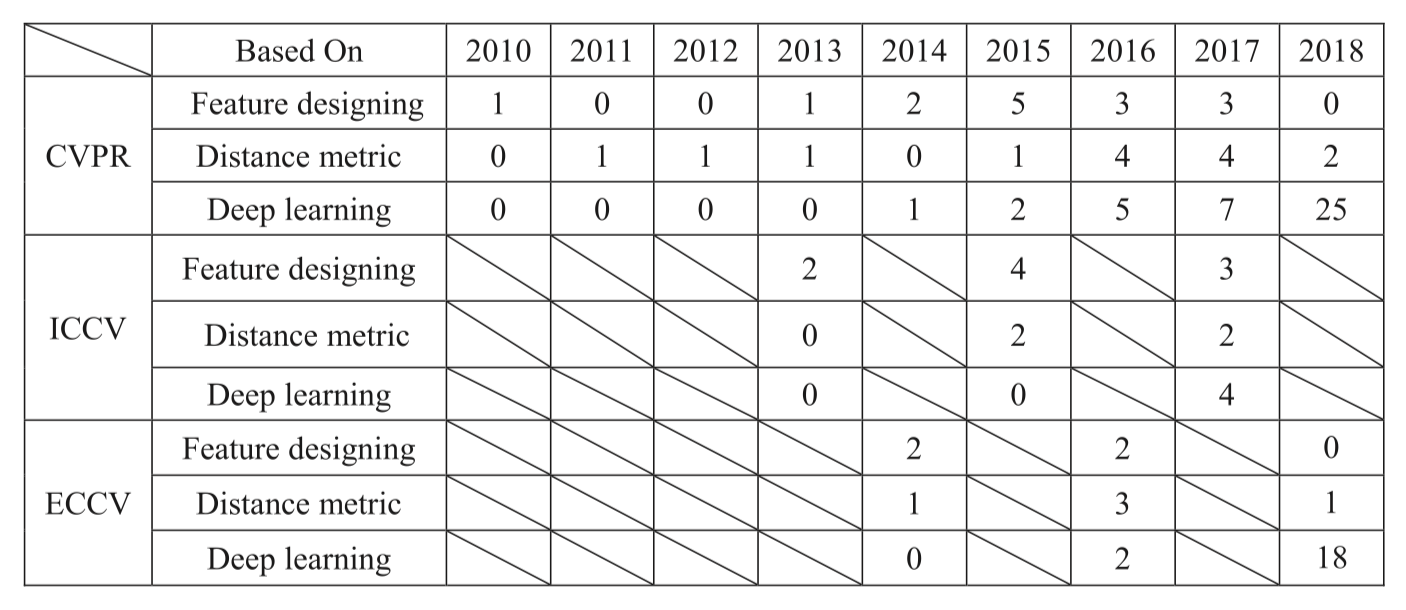
\includegraphics[width=\linewidth]{figures/papers_trend.png}
    \caption[Statistic of ReID related papers.]
    {The number of ReID papers depending on different approaches included by    
        the three top conferences in recent years
        ~\protect\cite{survey-on-dl-for-reid-2019}.}
    \label{fig:papers-trend}
\end{figure}

In this section, we are going to review the existing deep learning-based 
approaches for the person ReID task, most of them can be sorted into the 
following categories \cite{survey-on-dl-for-reid-2019}:

\begin{itemize}
    \item Identification model
    \item Verification model
    \item Distance metric-based model
    \item Parts-based model
    \item Others
\end{itemize}

We will go deeper into each of these different models in the following
subsections, but mainly concentrate on the identification model and the
distance metric-based model. Because our implementation which will be
introduced in the next chapter is a combination of these two models.

\subsection{Identification Model}
\label{sec:related-work-re-id-idm}

Identification model regards the ReID task as a classification task, distinct
identities will be seen as different classes, the basic architecture of the 
model is shown as \autoref{fig:id-model}. The input to the
network is the output from some kind of person detector. Then the deep
neural network (e.g. CNN) serves as a feature extractor. By making use of 
these extracted features the input image is tagged with an identity.

Due to the lack of data, the main issue of the classification model in deep
learning is always overfitting which means that the model performs well 
on the training set but poor on the validation set. Especially on the person 
ReID task, we want more training samples for each individual but most of the 
dataset only have few sample per instance (e.g. VIPeR only contains two images 
per identity). A lot of work have been done to solve this problem, they can  
roughly be categorized into
(1) add other constraints to revise overfitting and
(2) apply data augmentation techniques or create a larger dataset.

\begin{figure}
    \begin{center}
    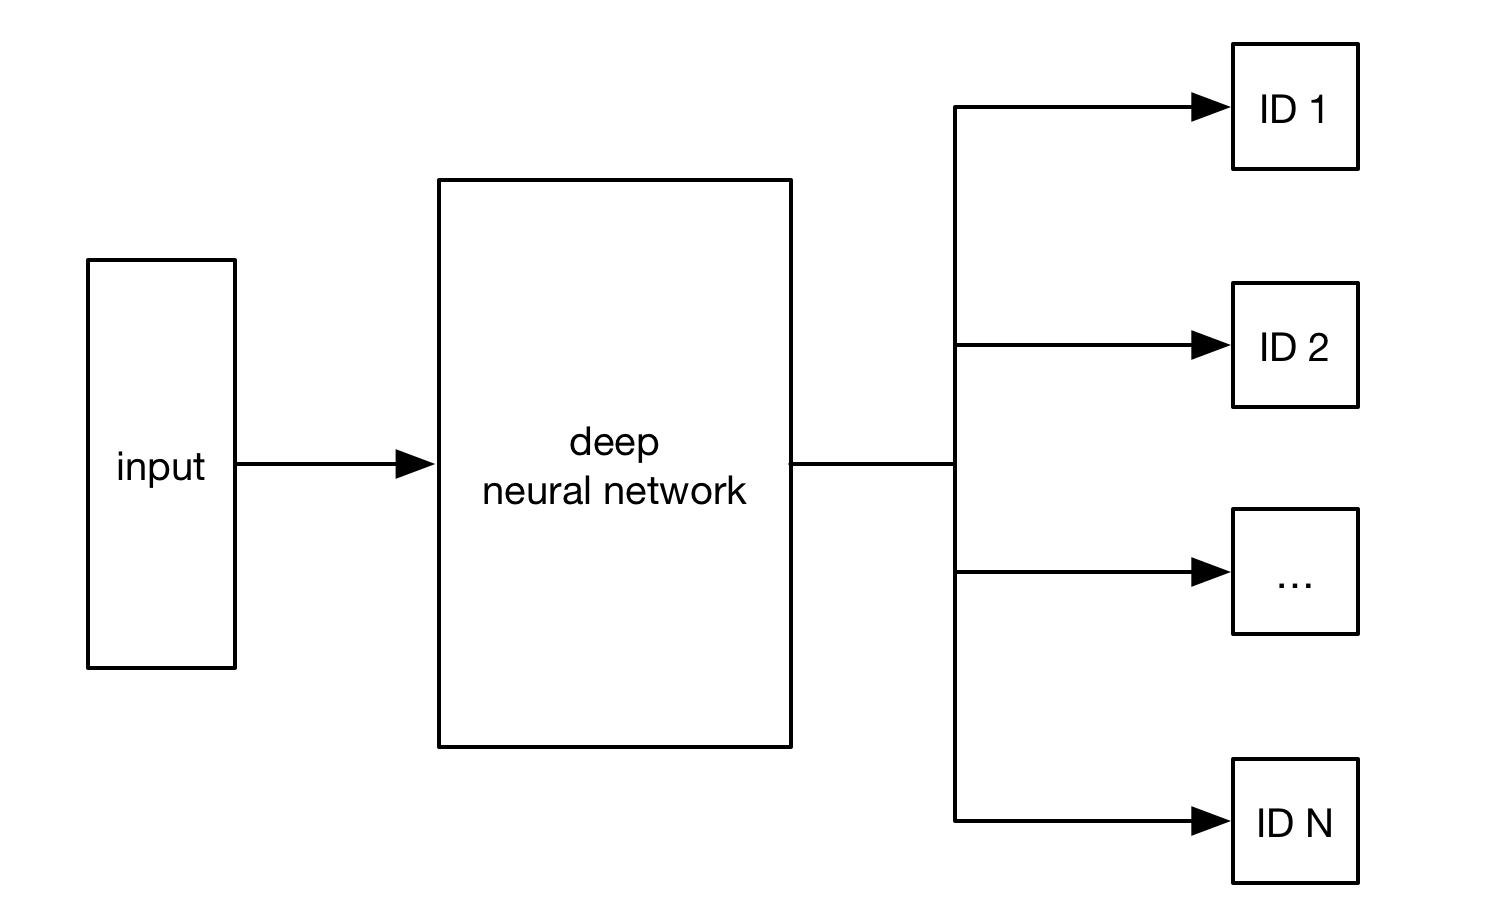
\includegraphics[scale=0.8]{figures/id_model.png}
    \end{center}
    \caption{Architecture of identification model.}
    \label{fig:id-model}
\end{figure}

In \cite{feature-fusion-net-2016}, the authors proposed a fusion feature
network (FFN) which can take both the CNN and the hand-crafted 
features into consideration at the same time, its architecture can be shown as
\autoref{fig:ffn}. FFN takes the identity image as input then branches into two
paths. 
For the CNN feature, five layers convolutional network and two fully 
connected layers were employed. For hand-crafted feature extraction, the 
original image was divided into horizontal stripes then color spaces and 
texture filters were applied in order to extract histograms which finally would 
be concatenated to form a feature vector. 
In the end, theses two kinds of features would be linked together through 
another dense layer. The whole network was trained under the guidance of 
a cross-entropy loss function and the classification result
was obtained from a softmax activation function 
\footnote{softmax is a function that takes as input a 
vector of $K$ real numbers, and normalizes it into a probability distribution 
consisting of $K$ probabilities. \cite{wikipedia-software-framework}} 
and during back-propagation parameters update would
also be constrained by the hand-crafted feature \footnote{hand-crafted feature 
is the feature designed beforehand by human experts to describe a set of  
characteristics of a specific object 
\cite{handcrafted-vs-deep-learning-features}.}.

\begin{figure}
    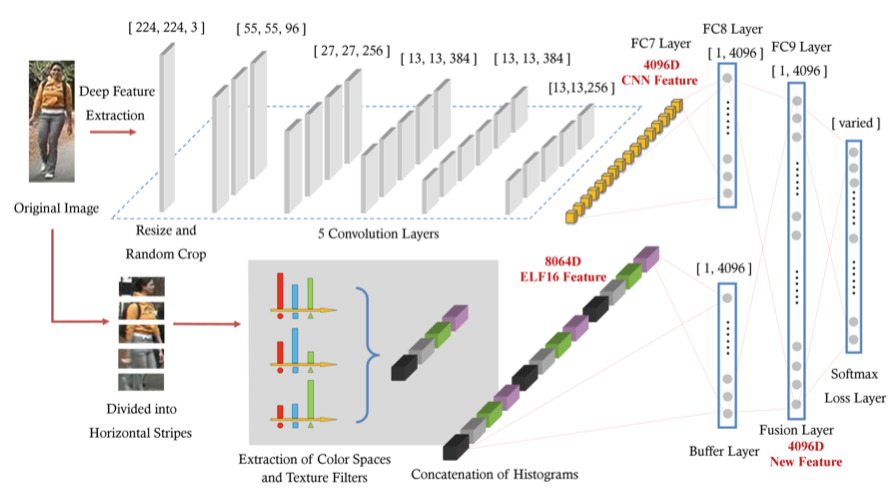
\includegraphics[width=\linewidth]{figures/ffn.png}
    \caption{
        Architecture of fusion feature network 
        ~\protect\cite{feature-fusion-net-2016}.
    }
    \label{fig:ffn}
\end{figure}

The idea behind classification model is to use several 
hyperplanes to separate different identities in the feature spaces. But since 
it is a high dimensional space, in some cases, the intra-class variance may 
larger than inter-class variance which is not a good property for a 
classification model.
In order to enhance the learned discriminative feature,
a hybrid network architecture that combined 
the Fisher vectors which include color histograms and SIFT and a deep 
neural network has been proposed in \cite{hybrid-net-lda-2016}.
%In our implementation, we also target to solve this problem,
%\cite{center-loss-2016}
%which originally proposed for face recognition called ``center loss"
%was employed. It maintains a center point of each identity
%and pushes each image embedding to its corresponding center so the
%variation between the same identity embedding is smaller.

It is worth to mention that as deep learning in person ReID area becomes more 
and more popular, there are several large datasets like
\cite{dataset-cuhk03-2014}, \cite{dataset-market1501-2015}, 
\cite{dataset-dukemtmc-2016} and \cite{dataset-cuhk03-np-2017} that have been 
released as well as their corresponding evaluation protocols.
Since deep learning methods really depends on data, these datasets do help the 
community a lot. With such large datasets, we are able to train the 
network directly based on the plain classification model. 
\cite{generic-deep-feature-for-reid-2016} trained the plain classification
network on multiple datasets with domain-guided dropout \footnote{Dropout is an 
implementer-friendly but useful technique  to prevent overfitting proposed
by \cite{dropout-paper-2014}.} strategy aiming at 
obtaining a cross-domain model. 

Jointly learning is another hot topic in the deep learning community, it means the model is trained under
the guidance of two or even more loss (objective) functions. In specific person 
ReID research, \cite{comb-id-and-center-loss-2017} proposed a jointly learning 
method which adopted identification loss and center loss 
\cite{center-loss-2016} at the same time, its architecture is shown as
\autoref{fig:comb-center-id-loss}. It claims that it is more efficient than the
pairwise or triplet model and the performance is also better by using their 
feature reweighting layer (FRW). The core idea is that during the training 
time, the model tries to enlarge the inter-class variation
and reduce the intra-class variation supervised by the center loss while
the identification loss makes full use of the image label compared with the 
verification model which just used the weak label information.

\begin{figure}
    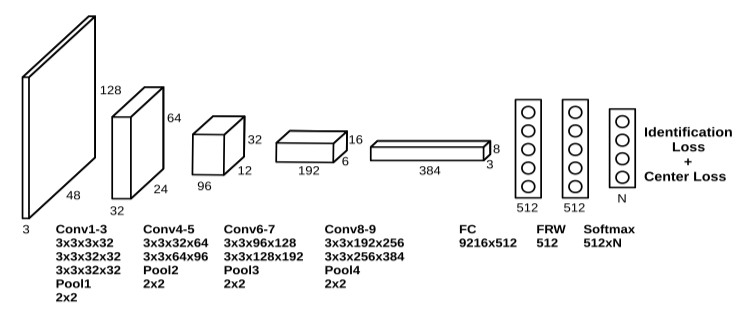
\includegraphics[width=\linewidth]{figures/comb-center-id-loss.png}
    \caption{A proposed CNN architecture with ID loss and center loss.
        ~\protect\cite{comb-id-and-center-loss-2017}.}
    \label{fig:comb-center-id-loss}
\end{figure}

\subsection{Verification Model}

Verification Model can be seen as a classification problem as well but it is a 
binary version. It takes a pair of images as input and output a similarity 
value indicating whether the paired images is the same person or not. Its 
architecture can be shown as \autoref{fig:vft_model} and simply formulated as:

$$
f(x_1, x_2) =
\begin{cases}
1,&  y_1 = y_2 \\
0,&  y_1 \neq y_2
\end{cases}
$$

\begin{figure}
    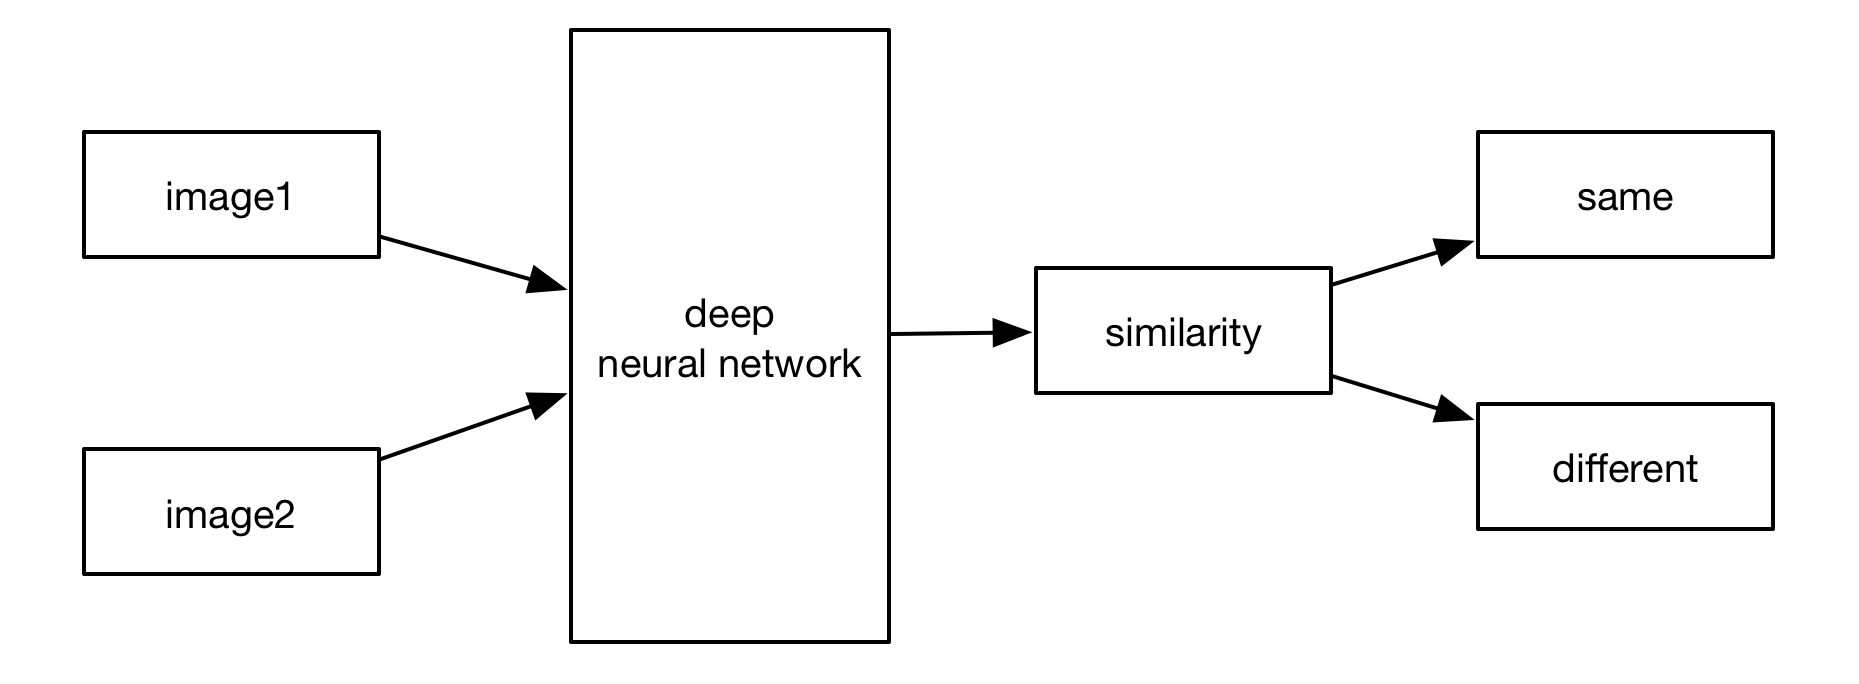
\includegraphics[width=\linewidth]{figures/verification_model.png}
    \caption{Architecture of verification model.}
    \label{fig:vft_model}
\end{figure}

The first verification model to address ReID task named filter pairing
neural network (FPNN) \cite{first-pairwise-net-for-reid-2014} was proposed in 
2014. Max-out pooling layers and patch-matching were employed to jointly handle 
geometric transforms and photometric, misalignment, background clutter and 
occlusions which are common issues in ReID domain.
At the time where datasets were still extremely limited, ``Siamese" deep 
network for metric learning which was firstly
proposed by \cite{first-siamese-net-for-reid-2014} was used to target this problem. 
Like the common verification model, it takes an image pair as input then pass 
them through three shared parameters but independent convolutional networks to 
perform operations on three non-overlapping parts of the images. The extracted 
feature descriptor will be flattened by a dense layer then used to
compute the cosine distance which would be converted into a similarity value. 
If the value is greater than a hyper-parameter threshold then the input pair 
will be considered as the same identity, otherwise different.
Based on the previous two works, \cite{an-improved-dl-archit-2015} comes up 
with an improved architecture shown as \autoref{fig:cvpr15_model} that include 
a layer to calculate cross-input neighborhood differences which is based on 
mid-level features to capture local relationships of the input paired images.

\begin{figure}
    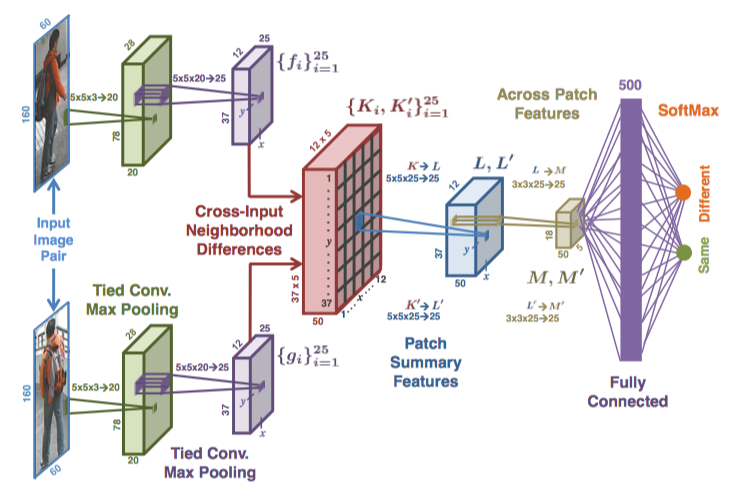
\includegraphics[width=\linewidth]{figures/cvpr15_model.png}
    \caption{Architecture proposed by ~\protect 
        \cite{an-improved-dl-archit-2015}.}
    \label{fig:cvpr15_model}
\end{figure}

But the verification models introduced above all have a common problem which is 
that the neural network employed by them are relatively
shallow. By this limitation, they did not benefit from digging the features 
which are discriminative enough to distinct different identities.
Besides, since we have to construct the image pair for training, there will be 
overhead added compared to the identification model. One more
thing is that the verification models only use the weak dataset label, which 
means that for a specific identity instance pair, it doesn't
care about their actual identity but they are the same or not. Unlike the 
identification model, it will tell directly which identity it is for each
given input.

Because of these limitations, only using the verification model may not achieve 
high accuracy in ReID task. Still, it is worth to mention
that the combination of identification and verification model can reach a 
promising result, \cite{id-verif-combined-learned-cnn-embedding-for-reid-2016} 
proposed such a model and comprehensively compared the advantages and 
disadvantages of these two models. They replaced contrastive loss by 
cross-entropy loss which is different from its sibling network on face 
recognition, then applied dropout regularization to prevent overfitting.

\subsection{Distance Metric-based Model}
\label{sec:related-work-re-id-dism}

The distance metric-based model aims at making the distance between the same 
identity as small as possible while keeping the distance between distinct 
identities as large as possible. 
One of the most popular used approach is the triplet architecture.
A triplet unit of images can be defined as:
$I_i=\{I_i^1, I_i^2, I_i^3\}$,
where $I_i^1$ called anchor, $(I_i^1, I_i^2)$ is positive pair and $(I_i^1, I_i^3)$ is negative pair.
For each triplet unit, the model will try to satisfy the following:

\begin{equation}
    \label{eq:triplet-model-goal}
    \norm{F(I_i^1) - F(I_i^2)} ^2 < \norm{F(I_i^1) - F(I_i^3)} ^2
\end{equation}

\noindent where $\norm{}^2$ means the L2 norm and $F(I)$ denotes the features 
learned by the model. Based on \autoref{eq:triplet-model-goal}
we can define the loss as following:

\begin{equation}
    \label{eq:common-triplet-loss}
    L(I) = \sum_{i=1}^{n} \max\{ \norm{F(I_i^1) - F(I_i^2)} ^2 - \norm{F(I_i^1) - F(I_i^3)} ^2, C \}
\end{equation}

\noindent where $C$ is a non-negative constant, guided by 
\autoref{eq:common-triplet-loss}, the network will be forced to maximize the 
distance between the anchor-positive and anchor-negative pair under L2 norm, 
the described procedure can be illustrated by \autoref{fig:triplet_objective}.

\begin{figure}
    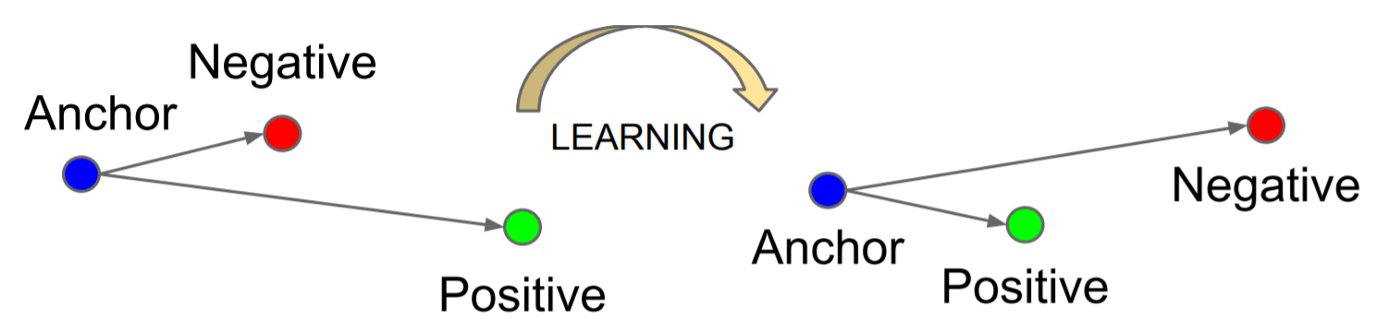
\includegraphics[width=\linewidth]{figures/triplet_objective.png}
    \caption{Objective of triplet loss ~\protect \cite{facenet-triplet-model}.}
    \label{fig:triplet_objective}
\end{figure}

In \cite{in-defense-of-triplet-loss-for-reid-2017}, comprehensive research had 
been conducted to the triplet model, covering the
strategy of sampling, different representations of the loss functions, 
comparison between pre-trained and plain model, etc. Some of their
methods are worth to mention:\\

\begin{itemize}
	\item They proposed a novel way to sample the triplet unit, in which randomly 
sampled $p$ identities within the whole training set and for
each selected identity randomly pick $k$ instances per mini-batch.\\
    \item They came up with several representations of loss functions, the most 
popular two of them are batch-hard loss $L_{BH}$ and batch-all loss $L_{BA}$.
As their name stated, batch-hard loss means to find the hardest triplet units
per batch and use them to contribute to the loss while batch-all loss 
means to use all the triplet units, no matter what they are, contributing 
to the loss. They can be formulated as \autoref{eq:batch-hard}.

\begin{equation}
\label{eq:batch-hard}
     L_{BH} = \sum_{i=1}^{P} \sum_{a=1}^{K}
            [
                m + \max_{p=1...K} D(f_{\theta}(x_{a}^i), f_{\theta}(x_{p}^i))
                - \min_{\substack{j=1...P\\ n=1...K\\ j\neq i}}
                D(f_{\theta}(x_{a}^i), f_{\theta}(x_{n}^j))
            ]_+
\end{equation}

\noindent where $D$ is a distance function, $f_\theta$ is the feature 
descriptor, $m$ is a margin constant, and $[\:]_+$ means the result within 
bracket will be a non-negative number.

\begin{equation}
\label{eq:batch-all}
    L_{BA} = \sum_{i=1}^{P} \sum_{a=1}^{K}  \:
             \sum_{\substack{p=1\\ p\neq q}}^{K} \:
             \sum_{\substack{j=1\\ j \neq i}}^{P} \:
             \sum_{n=1}^{K} \:\:
             [m + d_{j, a, n}^{i, a, p}]_+
\end{equation}

$$d_{j, a, n}^{i, a, p} =  D(f_{\theta}(x_{a}^i), f_{\theta}(x_{p}^i)) - D(f_{\theta}(x_{a}^i), f_{\theta}(x_{n}^j))$$

Effectively, by using $L_{BH}$ we can have $PK$ units contributing to the loss 
while using $L_{BA}$ we have $PK(PK - K)(K - 1)$ units
contribute to the loss. It really depends on the realistic scenario to 
determine which loss we should choose. At this point, it is
significant to note that these two variations of the loss still respect to the 
standard triplet loss function \autoref{eq:common-triplet-loss}.

\noindent 
\item During the training, they found that using the non-squared Euclidean 
distance is more stable than the squared one which will make the
optimization more prone to collapsing and reduce the interoperability of the 
margin constant (cannot be absolute distance any more).
\end{itemize}

\subsection{Parts-based Model}

A hand-crafted part-based model has been proposed for matching 
two persons based on their appearance \cite{hand-crafted-part-based}.
It partitioned a person into horizontal stripes to extract color and texture 
features. After this work, several other researchers \cite{part-based-pictorial-structure, part-based-triangle} employed more sophisticated strategies to 
divide a person into parts, but still based on hand-designed approaches. 
When deep learning comes to the picture, with the help of the
research on human pose estimation and landmark detection, the person ReID 
part-based model achieves several impressive results \cite{pose-driven-dcnn-for-reid, deep-part-based-glad, pose-invariant-embedding-for-reid}.

Attention mechanism is another milestone in the parts-based model, the current 
state of the art in person ReID task is 
produced by this model. 
In \cite{end-to-end-attention-network-for-reid}, the author first adopted
attention network to address ReID task, they proposed a LSTM-based
model using a recurrent approach that can output part attention feature 
dynamically for localizing discriminative regions of the pedestrian image. One 
year after, \cite{hpnet-attentive-deep-feature-for-reid} came up with a 
multi-directional attention mechanism for capturing multiple attention
information, the proposed network was named HP-Net.
For the part-based model, there is always a common issue which is the alignment 
problem. Once you divide the image into parts, how to align these chunks and 
calculate the similarity properly will be problematic. To address the 
misalignment issue, \cite{part-aligned-for-reid} introduced a CNN-based 
attention model that makes use of the distance between a paired image to
learn the part-feature for matching. In ECCV2018, \cite{pcb-and-rpp-for-reid} 
proposed a parted-based convolutional baseline model (PCB) which employed a 
simple uniform partition strategy and assembles part-informed feature into a 
descriptor and a refined part pooling (RPP) method which reinforces the 
within-part consistency introducing a large margin of improvement without 
requiring any part labeling information, the architecture is shown as 
\autoref{fig:rpp}. However, the part-based model still has its own limitations:

\begin{figure}
    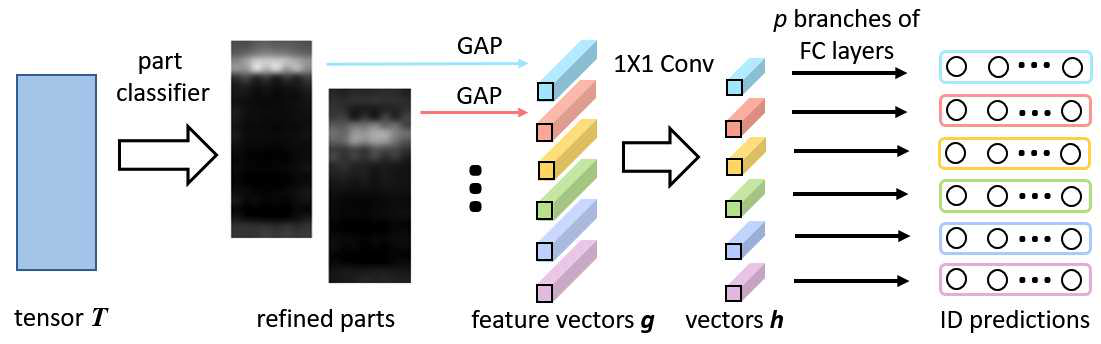
\includegraphics[width=\linewidth]{figures/rpp.png}
    \caption{PCB in combination of refined part pooling ~\protect \cite{pcb-and-rpp-for-reid}.}
    \label{fig:rpp}
\end{figure}

\begin{itemize}
    \item Adding part-based branches reduced the efficiency of the model.
    \item Most attention-based model only considers region-level attention and 
    discard the pixel-level saliency.
    \item Most of the models do not consider the spatial context information 
    between different part-based features.
\end{itemize}

\subsection{Others}
\label{sec:related_work_other}

Besides the four major models described above, there are still some other deep 
learning-based researches on ReID community.
Even with the datasets like CUHK03, Market1501, and DukeMTMC-reID, the average 
numbers of image per person is still quite limited. The first work tries to 
enlarge the dataset using a generative adversarial network (GAN) and was 
introduced by \cite{first-gan-for-reid}. They employed GAN to generate 
unlabeled samples and adopted a CNN to extract feature for representation 
learning. Then label smoothing regularization is used for outliers method.

A camera style adaption model to adjust the CNN training was proposed in 
\cite{camera-style-adaptation-for-reid}. 
More precisely, CycleGAN is used to transfer the style of images captured by 
one camera to another. Given an image from camera No.1, the model
can produce the image which looks like captured by camera No.2.

Unlike most of the works which are based on RGB image, it is noteworthy to 
mention a work which employs RGB-D data as input.
A novel method for person ReID using RGB-D data was proposed in 
\cite{rgbd-for-reid}, their working pipeline can be shown as 
\autoref{fig:rgbd-pipeline}.
It took a RGB-D image as input, then performed a segmentation to obtain 
different parts of the human body. By using this information, they
did 3D reconstruction and pose transformation resulting with a standard human 
3D model. Then using the attributes computed from
the 3D model to perform re-identification.

\begin{figure}
    \begin{center}
        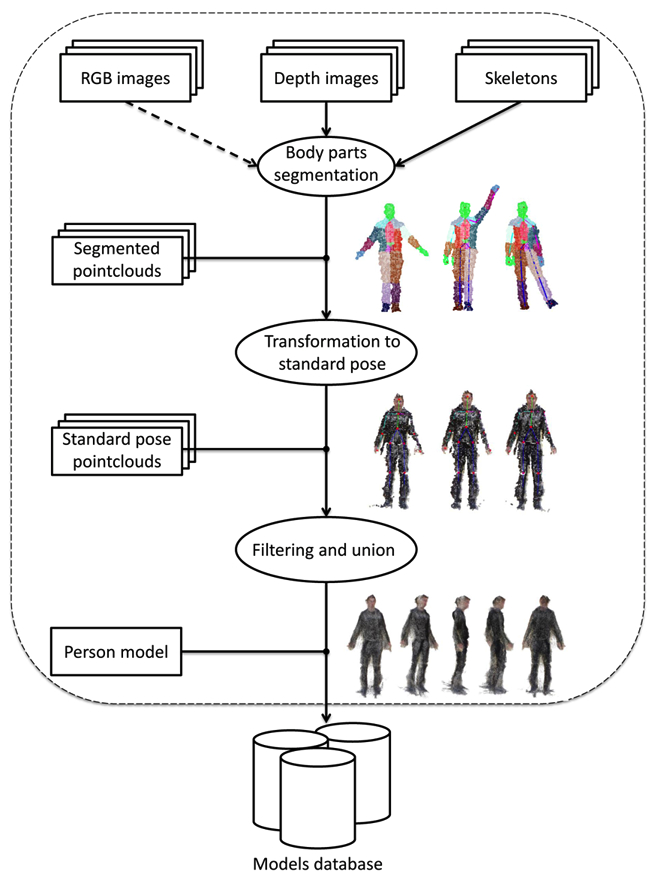
\includegraphics[scale=0.4]{figures/rgbd_for_reid.png}
        \caption{The working pipeline for ReID with RGBD data ~\protect \cite{rgbd-for-reid}.}
        \label{fig:rgbd-pipeline}
    \end{center}
\end{figure}

%\section{OpenISS Framework}
\section{Available Software}
\label{sec:related_work_framework}

To develop a general solution for (1) deep learning-based person 
re-identification and (2) device abstraction, from the implementation point of 
view, we have to survey the currently available software that may be useful for 
our solution.

\subsection{Freenect and Freenect2}
\label{sec:related_work_openiss_freenect}
The most impressive depth camera to people nowadays may still be the Microsoft 
Kinect, even if it has been dropped by its own company now. It was the first 
consumptive depth camera in the market released in November 2010. Kinect was
designed for Microsoft Xbox 360, a video game console. In order to let the game 
designer to fully make use of it, a corresponding closed source library (known 
as Microsoft Kinect Developer Toolkit) was also released to enable the 
programmability of the device.

Since the Microsoft Kinect Developer Toolkit is closed source and can only be 
used on Windows machines. A group of people from the community made an 
open-source driver for Kinect named Freenect to enable it works on Linux, MacOS
and Windows. By using this Freenect driver, people can obtain the raw depth 
data from the device directly. A lot of researches based on depth data has 
been based on this solution. When Microsoft released Kinect v2 (the second version
of Kinect), the community also came up with the driver Freenect2 with the same 
functionality.

\subsection{OpenNI2}

OpenNI or Open Natural Interaction library was originally created by PrimeSense 
which is a depth-sensing solution provider company. Kinect was using their 
technology to obtain the depth data from the sensors. After the
acquisition of PrimeSense by Apple, they shut down the official website but the 
community (like Occipital and other former partners) is still keeping a forked 
version of OpenNI2 active as an open-source library for their product.

By using the OpenNI2 framework, we can perform the following operation using the
same unique APIs, if the hardware driver respects the OpenNI2 standard.
Fortunately, both Freenect and Freenect2 have the option to build an 
OpenNI2-supported version of them:

\begin{itemize}
    \item Voice and voice command recognition.
    \item Hand gestures.
    \item Body motion tracking.
\end{itemize}

\subsection{OpenCV}

OpenCV is a library of programming functions mainly for computer vision. It
was originally created by Intel (for image processing) in 2000 and now lead by
Itseez. The library is cross-platform and open source under the BSD license,
widely supports most of the existing operating systems. The library was 
originally written in C, but since 2009 it primarily changed to C++. Nowadays, 
it also adds CUDA-based and OpenCL-based GPU calculation, machine learning and
deep learning (TensorFlow, Torch/PyTorch and Caffe) support.

\subsection{NiTE2}
\label{sec:related_work_openiss_nite2}

NiTE2 is a piece of middleware of OpenNI2 library. It has to work with OpenNI2
underneath and provides more powerful functionality than OpenNI2 does. It uses 
the same design philosophy of OpenNI2 which is only supposed to provide the
infrastructure and leave all the other functionalities to the middleware.
Unfortunately, NiTE2 is a closed source library provided by PrimeSense, it was
written in C++ and only comes with the header files and the binary library. By
using NiTE2, we can get the following data:

\begin{itemize}
    \item Skeleton data of the tracked full human body.
    \item Gesture data of the tracked hand.
\end{itemize}

\subsection{RealSense SDK}

RealSense SDK is a cross-platform library from Intel for their own depth
cameras. It allows the developer to access depth and color streaming and
provide the basic camera parameters for calibration. Since the SDK is provided
by the manufacturer directly which means they know everything about the
hardware, it is more powerful than Freenect and Freenect2 as to Kinect. The SDK
is written by C++ and hosted on GitHub. The
community is still quite active and they still try to add more functionalities
to the SDK (like support OpenNI standard, working with OpenCV library, provide
more wrapper for other programming languages rather than C++).

\subsection{CPython}
\label{sec:related_work_cpython}

Our research team proposed the OpenISS framework, which is designed to be written in C++ since most of
its dependencies list above are in C++. But nowadays, most of the deep learning
programs are written in Python, and for experiment and prototyping purposes,
Python has a more efficient development environment. In order to invoke the
deep learning model from OpenISS framework, we need something to connect C++
and Python. CPython is our desired bridge, it is the reference implementation
of the Python programming language written in C and Python. It has a foreign
function interface with support to several other programming languages and C is
one of them. By making use of CPython we can exchange a class, a function, a
variable or other data structure with the languages on two sides of the bridge.

\subsection{TensorFlow}
\label{sec:related_work_openiss_tf}

Since deep learning got a lot of attention recently, there is a variety of deep learning
frameworks being developed. \autoref{fig:dl-frameworks} shows the popularity of
most of the existing platforms. Among these, one of the most famous is Google's 
TensorFlow \cite{tensorflow2015-whitepaper}, an open-source library written in C++. 
It is a symbolic math library that provides various kinds of
tensor operations for dataflow and differentiable programming. It uses
a computational graph with respect to the chain rule to perform
back-propagation which is the core concept for updating the parameters (or we
can say training). Also, TensorFlow can encapsulate the hardware differences and
support training on multiple GPUs if they are available without any code
modification. It is becoming more and more popular in the industry and production
environment.

\begin{figure}
    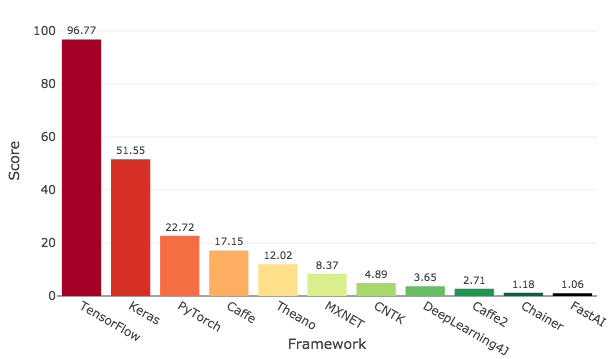
\includegraphics[width=\linewidth]{figures/dl_framework.png}
    \caption{Power score of the most deep learning frameworks in 2018
        ~\protect \cite{score-dl-framework}.}
    \label{fig:dl-frameworks}
\end{figure}

While TensorFlow is popular in the industry, another framework named Pytorch
gets more attention among academic users and researchers. In the ReID research 
community, most of the code is based on Pytorch. There is even no baseline
model implemented in TensorFlow and Keras for the ReID task.
In contrast, since YOLO is widely used in the industry, there are already numerous
existing implementations of YOLO in TensorFlow. In order to keep our
implementation consistent in one framework and reduce the overhead for
translating data from one to another, we chose TensorFlow as our deep
learning platform. By employing it, our research actually fills a gap, 
as no existing solution for ReID task is currently based on TensorFlow.


\subsection{Keras}

Keras \cite{keras-framework} is a high-level open-source library written in
Python, firstly developed by Francois Chollet, which can take TensorFlow,
Theano and some other frameworks as its back-end. It doesn't provide the
mathematics operation implementation as they were left to the backend but a
human-friendly APIs which can allow you to prototype your conceptual
neural network (or other machine learning architecture) easily and experiment
with different deep learning frameworks. TensorFlow adopted Keras into its core
and announced it as the official high-level APIs in 2017 and more support has been 
added to Keras since TensorFlow 2.0 which was released in 2019.

\section{Summary}

In this chapter, we gave an extensive review to the most common deep
learning-based methods in both object detection and person re-identification
domains.
%
For the object detection problem, we started from the seminal work R-CNN
and stated the key contributions of each existing approach and compared them
with similar methods if comparable. Due to our real-time limitation from the
requirement, we are restricted to use one-stage method. Precisely, we select
YOLO v3 as our detector, because its inference time is by a large margin better than
all the others and the community already has a lot of existing resources for it.
%
For person re-identification problem, we introduced a total of five different 
models and explained their network architectures and loss functions. Jointly 
considering the trade-off between implementation complexity and the model's 
performance, we decided to use a combination of the identification model and 
the triplet model.
%
In the last part of this chapter, we listed all the available
software that may be employed as dependencies in our work. In the next chapter, we 
will start to present our solution.

% EOF
